\documentclass[tikz, border=5pt]{standalone}
\usetikzlibrary{positioning, automata}

\begin{document}

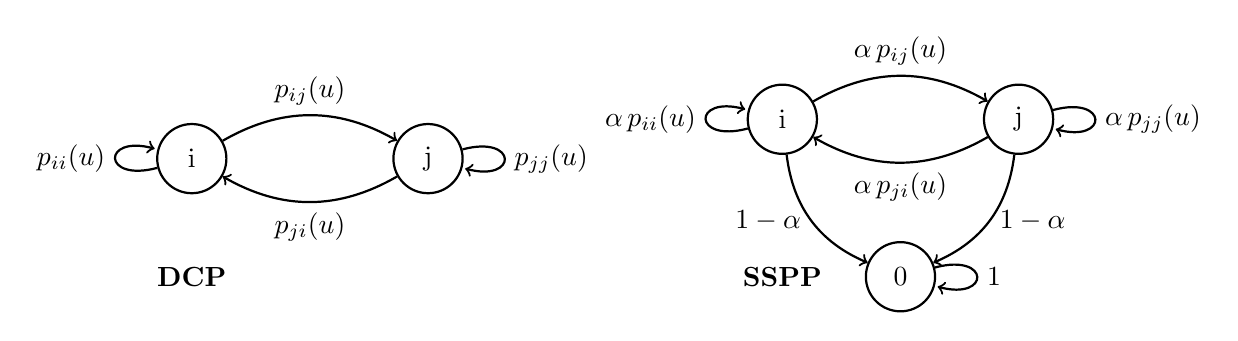
\begin{tikzpicture}
    %% DCP
    \begin{scope}[yshift=-0.5cm]
        % States
        \node[state, thick] (i) at (0, 0) {i};
        \node[state, thick] (j) at (3, 0) {j};

        % Transitions
        \path[->, thick] (i) edge [bend left, above] node {\( p_{ij}(u) \)} (j);
        \path[->, thick] (j) edge [bend left, below] node {\( p_{ji}(u) \)} (i);
        \path[->, thick] (i) edge [loop left] node {\( p_{ii}(u) \)} (i);
        \path[->, thick] (j) edge [loop right] node {\( p_{jj}(u) \)} (j);

        % Labels
        \node (l) at (0, -1.5) {\textbf{DCP}};
    \end{scope}

    %% SSPP
    \begin{scope}[xshift=7.5cm]
        % States
        % States
        \node[state, thick] (i) at (0, 0) {i};
        \node[state, thick] (j) at (3, 0) {j};
        \node[state, thick] (0) at (1.5, -2) {0};

        % Transitions
        \path[thick, ->] (i) edge [bend left, above] node {\( \alpha \, p_{ij}(u) \)} (j);
        \path[->, thick] (j) edge [bend left, below] node {\( \alpha \, p_{ji}(u) \)} (i);
        \path[->, thick] (i) edge [loop left] node {\( \alpha \, p_{ii}(u) \)} (i);
        \path[->, thick] (j) edge [loop right] node {\( \alpha \, p_{jj}(u) \)} (j);
        \path[->, thick] (i) edge [bend right, left] node {\( 1 - \alpha \)} (0);
        \path[->, thick] (j) edge [bend left, right] node {\( 1 - \alpha \)} (0);
        \path[->, thick] (0) edge [loop right] node {\( 1 \)} (0);

        % Labels
        \node (l) at (0, -2) {\textbf{SSPP}};
    \end{scope}
\end{tikzpicture}
\end{document}
